\customHeader{0}{Practical Implications}
\label{08_practical_implications}

\customHeader{1}{Overview}
\label{08_overview}


After obtaining the hyperparameters for training the best classifiers (Table \ref{tab:07_best_classifiers}), the \gls{pesv} team will include our results into their data collection pipeline, as part of the \gls{tiersesv} project.

We implement two services for the \gls{tiersesv} project:
\begin{itemize}
    \item An inference service.
    \item A training service.
\end{itemize}



\customHeader{1}{Inference Service}
\label{08_inference_service}


\begin{figure}[h]
    \centering
    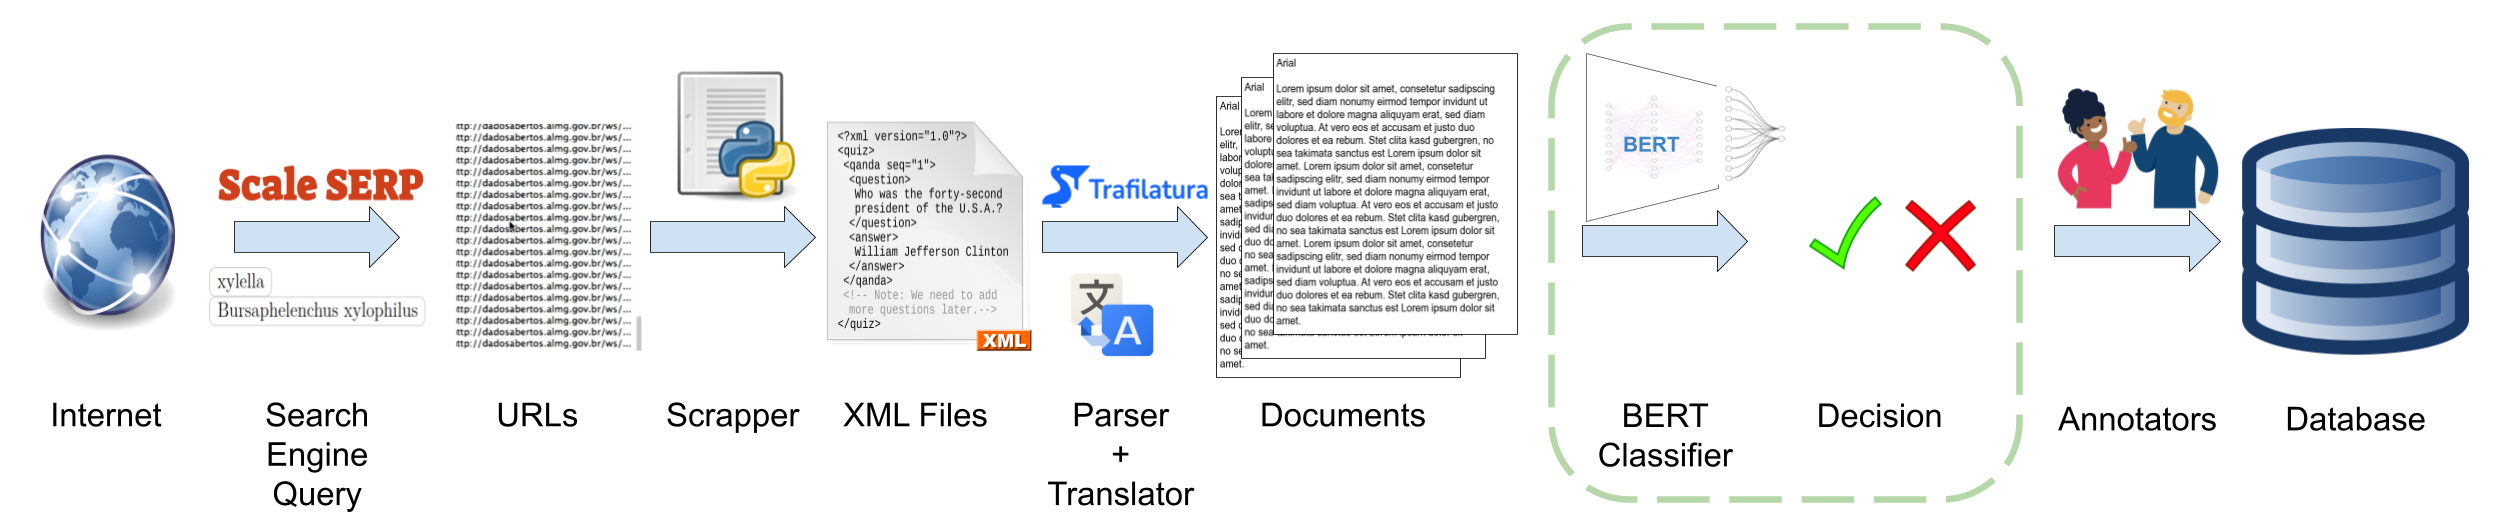
\includegraphics[width=\textwidth]{Figures/08/08_vsi_dataset_collection_with_classifier.png}
    \caption{Our classifiers added to the \VSI{} Data Collection Pipeline}
    \label{fig:08_vsi_data_collection_pipeline_with_classifier}
\end{figure}


We assemble a filter consisting of two modules:
\begin{enumerate}
    \item Heuristics 
    \item Neural \textclassification{}
\end{enumerate}

The heuristics module helps discard entries without content. For \textclassification{}, the filter applies our models to the documents with content.

The filter's output will be incorporated into the \gls{vsi} database, and in general, we expect it to alleviate the workload for the \gls{vsi} experts.

The implementation of this filter will be done using the Python package made for this thesis. 

\begin{enumerate}
    \item First, the scrapping results fed to the tool we developed to extract the \trafilaturaTitle{}, \trafilaturaAbstract{}, \trafilaturaFulltext{}, and the \translationTitle{}.

    \item Then, the noise (HTML tags, URLs, etc) is removed from the text, for each \contentType{}
    
    \item Afterward, the heuristics' module uses the tools developed during preprocessing. By exposing the functions used to detect error messages and scrapping failures, we can discard documents without content.


    \item  Then, for each \contentType{}, the cleaned text is given as input for the \textclassification{} model.

    \item Finally, the output of the filter for a particular document consists of
    \begin{itemize}
        \item A boolean indicating whether the document was discarded.
        \item The cleaned text
        \item The prediction: Relevant VS Irrelevant
        \item The label probabilities
    \end{itemize}


\end{enumerate}

By considering the observations about deleting error messages and handling scrapping errors (\headerName{}s \ref{vsi_deleting_error_messages} and \ref{05_vsi_handling_scrapping_errors}), we can expect the heuristics model to discard from 20\% to 30\% of unique documents, depending on the \contentType{}.

This filter will be used for inference on the documents scrapped every week by the \gls{pesv} Platform. For easy of use, it will be implemented using a \texttt{REST} API, running on the \MAIAGE{} servers, and added to the \href{https://bibliome.github.io/alvisnlp/)}{\emph{AlvisNLP-ML}}\footnote{\url{https://bibliome.github.io/alvisnlp/)}} suite of the \bibliome{} group \myparencite{alvisnlp}.
Finally, when publishing selected documents to the official bulletin of the   \gls{pesv} Platform, these will be ordered by descending relevance.



\customHeader{1}{Training Service}
\label{08_training_service}

As more entries are added to the \gls{vsi} database, it will become necessary to update the models used for \textclassification{}. This is handled by the training service, which implements the complete pipeline for training the best performing classifiers (Table \ref{tab:07_best_classifiers}).

The \gls{vsi} experts will have to decide on the frequency and data to be used for training. 
That is, if the training is done every week, or every two or three weeks. Also, if, as their interests change over time, it would be more convenient to restrict the data used for training, for example, using only the last two or three months.

The training service should be executed on the \texttt{Lab-IA} cluster. The scripts for the training service are available in our GitHub repository.



\customHeader{1}{Consequences for Plant Health Monitoring}
\label{08_consequences}

Up to now, the \gls{vsi} experts at the \gls{pesv} Platform have been manually revising every scrapped document. Including \textclassification{} into the annotation pipeline will alleviate the workload of the \gls{vsi} experts, helping with Plant Health Surveillance in the long term.

Including the Heuristics module will allow the \gls{vsi} experts to know which queries and websites are problematic for their scrapping tools. 

Given that the \gls{vsi} experts will read the documents flagged as Relevant by our system, we decided to calculate the ratio of positives for the best classifiers on their test splits. Also, we prefer lower rates of false negatives, that is, the proportion of documents that are actually Relevant but that our system flags as Irrelevant (Table \ref{tab:08_ratio_of_positives}).


\begin{table}[ht]
\centering
\begin{tabular}{ccccc}
\hline
  \contentType{}                                   & Model & Training Method & Positives/Total & FN/Total \\ \hline
  \trafilaturaTitle{} & \bertmultilingual{} & \petThousand{}  & 43.33\% & 2.0\%\\ \hline %0.43333333333333335 \\

 \trafilaturaAbstract{} & \bertxlmroberta{} & \petThousand{} & 40.16\% & 2.23\% \\  \hline %0.4016489988221437 \\
\trafilaturaFulltext{} & \bertmultilingual{} & \petThousand{} & 26.55\% & 1.66\%\\%0.29547471162378 \\ 
\trafilaturaFulltext{} & \bertxlmroberta{} & \balanced{} & 24.16\% &  2.89\%\\%0.24156305506216696 \\
\trafilaturaFulltext{} & \bertxlmroberta{} & \petThousand{} & 37.27\% & 1.20\% \\ %0.37267080745341613 \\
\hline
\translationTitle{} & \bertmultilingual{} & \petThousand{} & 34.62\% & 1.69\% \\ %0.34615384615384615 \\
\hline
\end{tabular}
\caption{Positives and FN ratios for the best classifiers}
\label{tab:08_ratio_of_positives}
\end{table}

The low False Negative rates mean that only 2 of 100 Relevant (unique) documents will be ignored by our systems, which we consider a great result. 
As mentioned in \headerName{} \ref{vsi_results_of_preprocessing}, the real balances in the \gls{vsi} Dataset range from 12\% to 14\% positives. The closest one of our classifiers approaches this percentage, the fewer documents the \gls{vsi} experts will have to manually revise.

In the best case, with a $24\%$ Positive ratio, the \gls{vsi} experts will be presented with around $76\% \approx 3/4$ fewer documents than now. In the worst case, with a $43\%$ Positive ratio, they will be presented $57\% \approx 1/2$ fewer documents. 

\putInBox{
This shows that including our system into their monitoring pipeline will substantially reduce the documents to be manually reviewed, enabling the \gls{vsi} experts to either review the same amount of documents in less time, to use the same time to review more documents, or to expand their surveillance to more pathogens. We consider this outcome to be satisfactory and a fitting conclusion to the project.
}


\clearpage


% Heuristics
% NLP

% noticing which websites are problematic for their tool

\iffalse


1. Dans le workflow de travail de la Plateforme ESV, il est déjà prévu un slot pour le filtrage automatique de documents.


    Search (Google) -> Extract (Proprietary) -> Extract (Trafilatura) -> Traduction titre (Google) [-> Filter (you)] -> Traduction fulltext (Google) -> Presentation (Proprietary, screenshot) -> Examination (Humans)


2. Le projet TIERS-ESV vise à étudier les apports possibles des technologies du NLP pour la veille épidémiologique. Participants: Bibliome, Migale, Plateforme ESV.


3. Le projet TIERS-ESV devra choisir un modèle pour l'étape de filtrage.

Critères:

    - performances: R/P/F1/F2 mais aussi balance entre Faux Négatifs (1/R) et Taux de Positifs ( (TP+FP)/N )

    - temps d'entraînement et d'inférence


3. Le projet TIERS-ESV fera de ce modèle un service:

    - entraînement et inférence automatisées
    
    - commandable à distance

    - fréquence: 1 semaine

    - décisions: fréquence d'entraînement, ensemble d'entraînement. Critères: temps d’entraînement, actualité deu filtrage par rapport à la perspective des agents. train with the last three months


4. Outils d'intégration

    - AlvisNLP (https://bibliome.github.io/alvisnlp/)

    - REST

    - Migale CPU farm


5. Conséquences

    - Présentation des documents rankés (positifs d'abord)

    - économie de travail pour les agents de la Plateforme ESV (Taux de Positifs), moins de temps à lire des docs => peuvent lire plus de docs => peuvent surveiller plus d'agents pathogènes => meilleure surveillance épidémiologique => en finir avec la faim dans le monde





\fi